\section{Data Analysis}
The following section will include an overview and visualisation of the data acquired for the research.

\subsection{Engine Health Monitoring Data} \label{sec:ehm}
The research was carried out on \ac{ehm} data. This data was recorded by sensors in 231 BR725 engines during a total of 14\,045 flights, and returned on a voluntary basis to Rolls-Royce by operators for analysis.

The BR725 is used in the Gulfstream G650, a business jet built for up to 18 passengers. Each G650 has two engines; to minimise the amount of data used, the values used in this thesis were taken from the left engine only.

\begin{figure}[t]
    \centering
    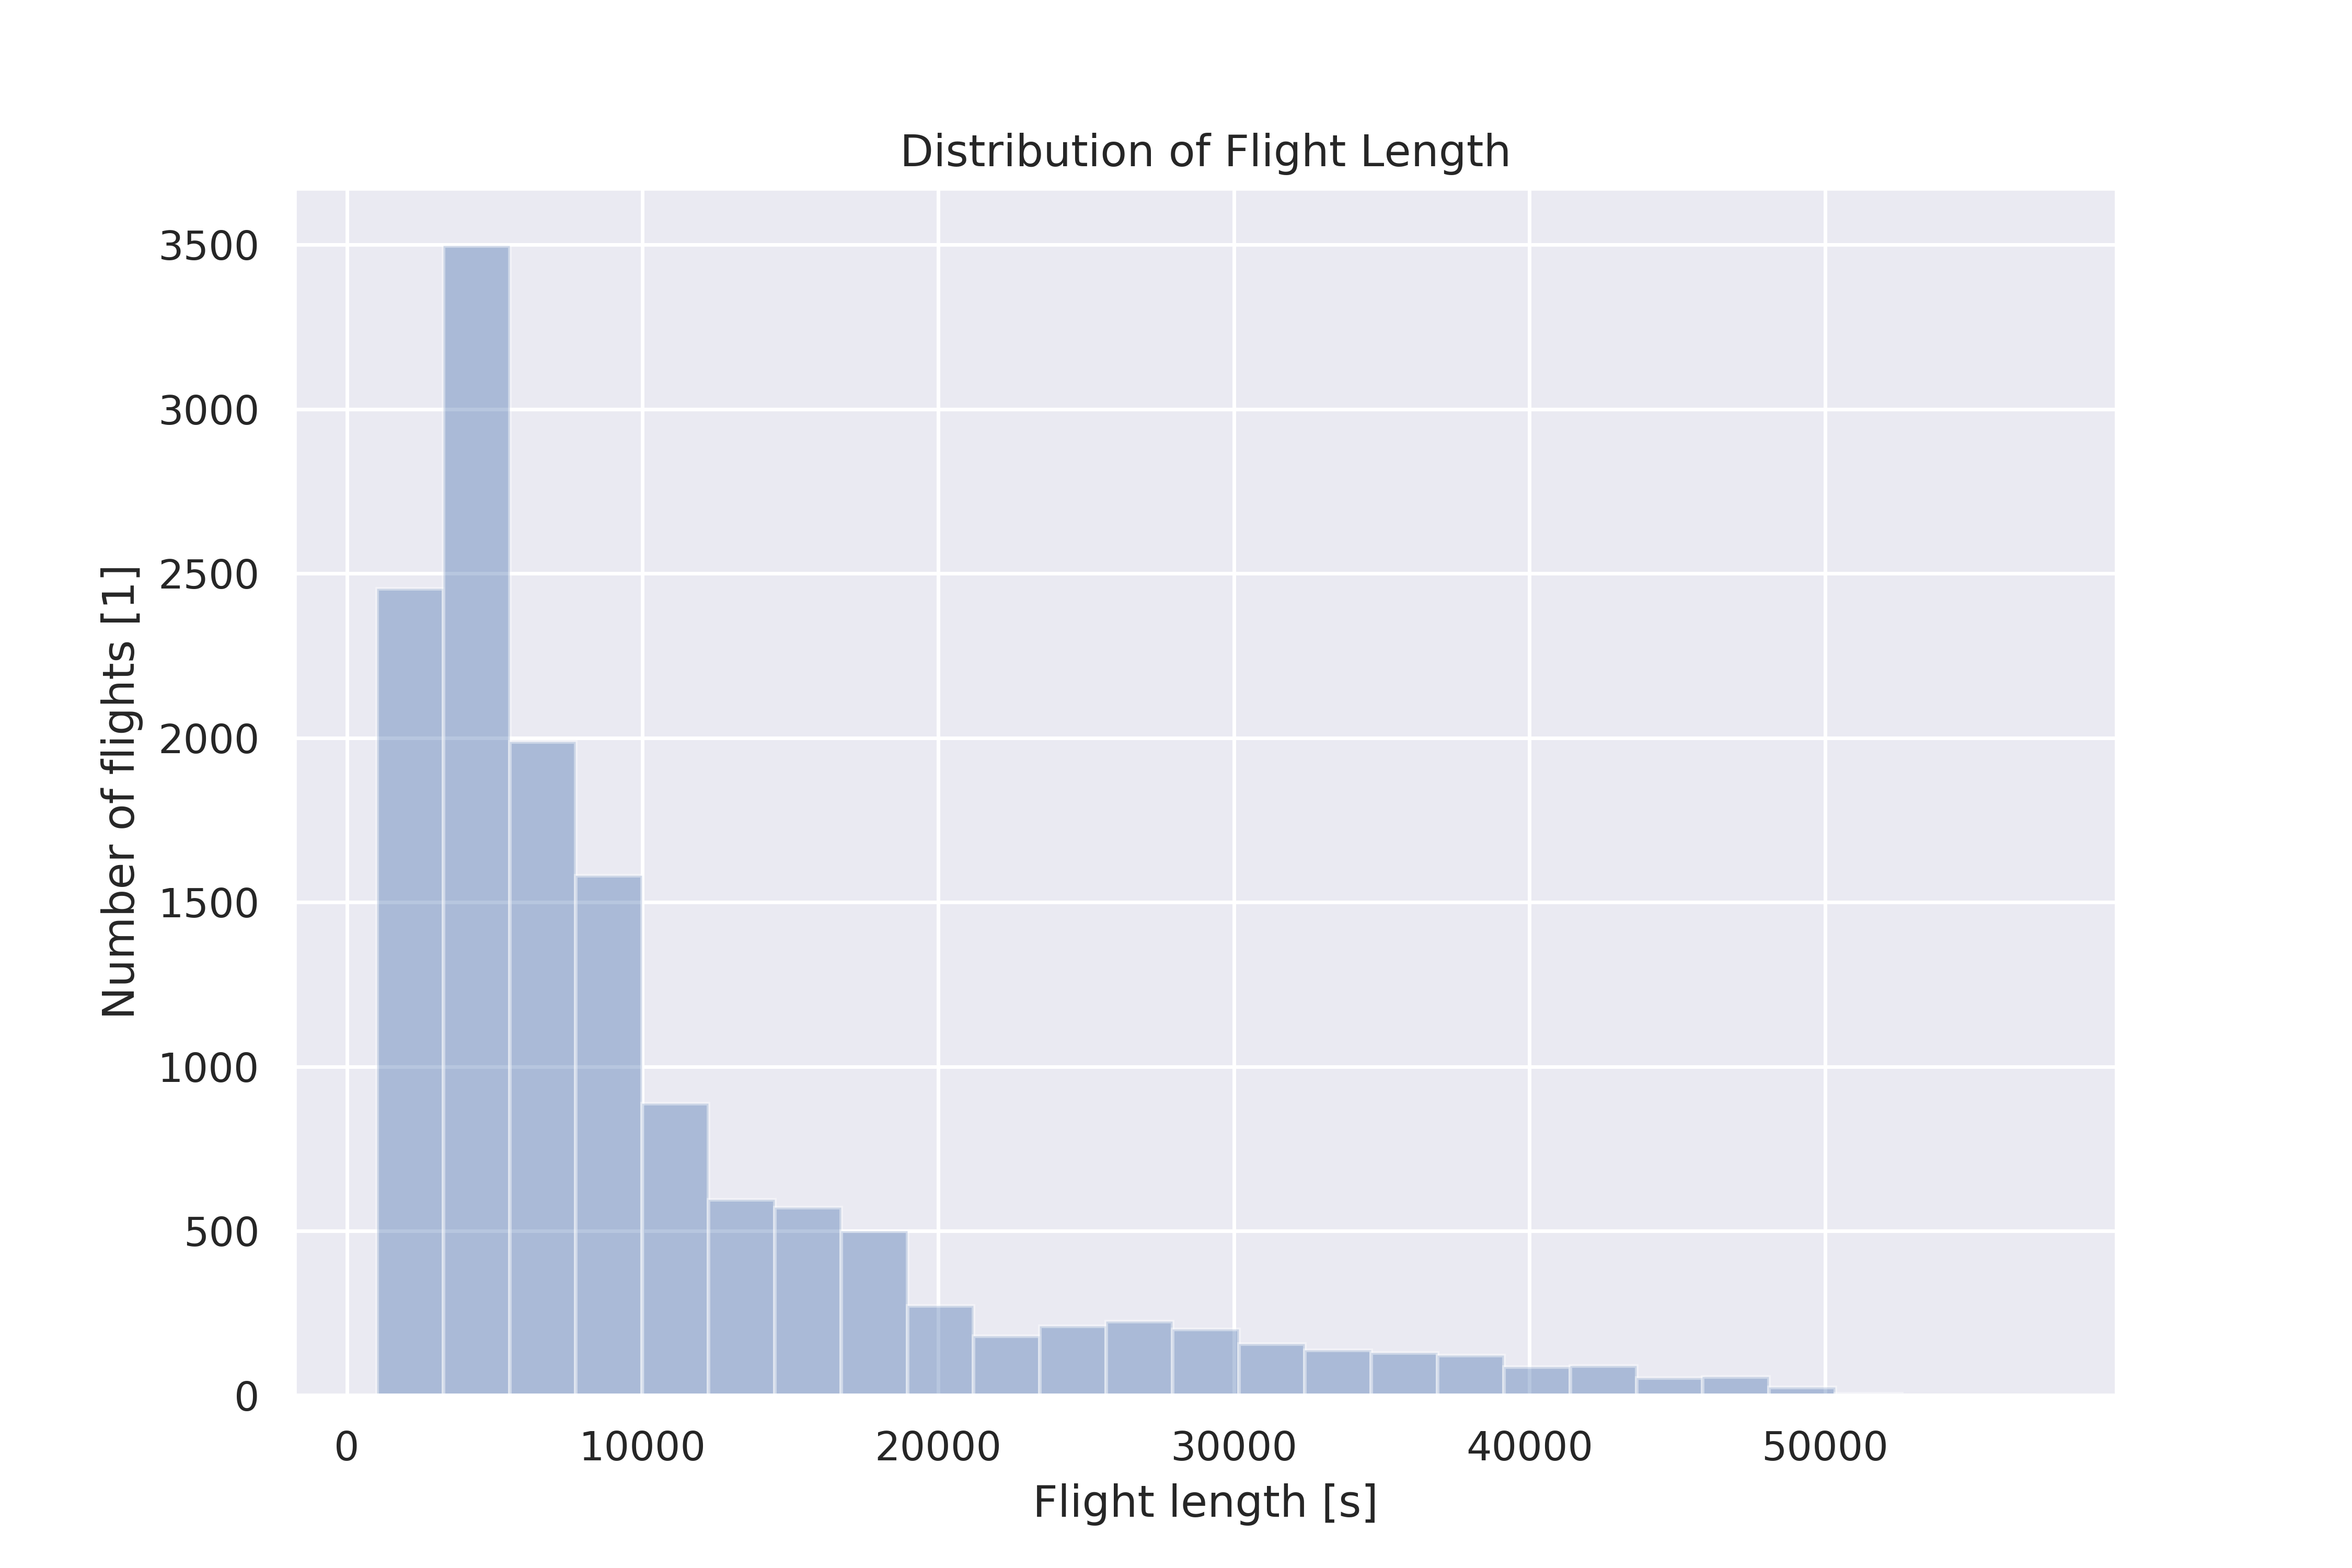
\includegraphics[width=0.95\textwidth]{length_hist}
    \caption{\label{fig:flight_len} A histogram of the lengths of 14\,045 flights}
\end{figure}

The flights range in length from 1\,013 to 57\,062 seconds (approximately 0.28 to 15.85 hours), with a mean length of 10\,182.82 seconds and a standard deviation of 9\,561.03 seconds (see Figure \ref{fig:flight_len}).

Each flight is summarised in a \ac{csv} file with 216 columns, comprising one timestamp and 215 values per second of recording time.

\begin{figure}[ht]
    \centering
    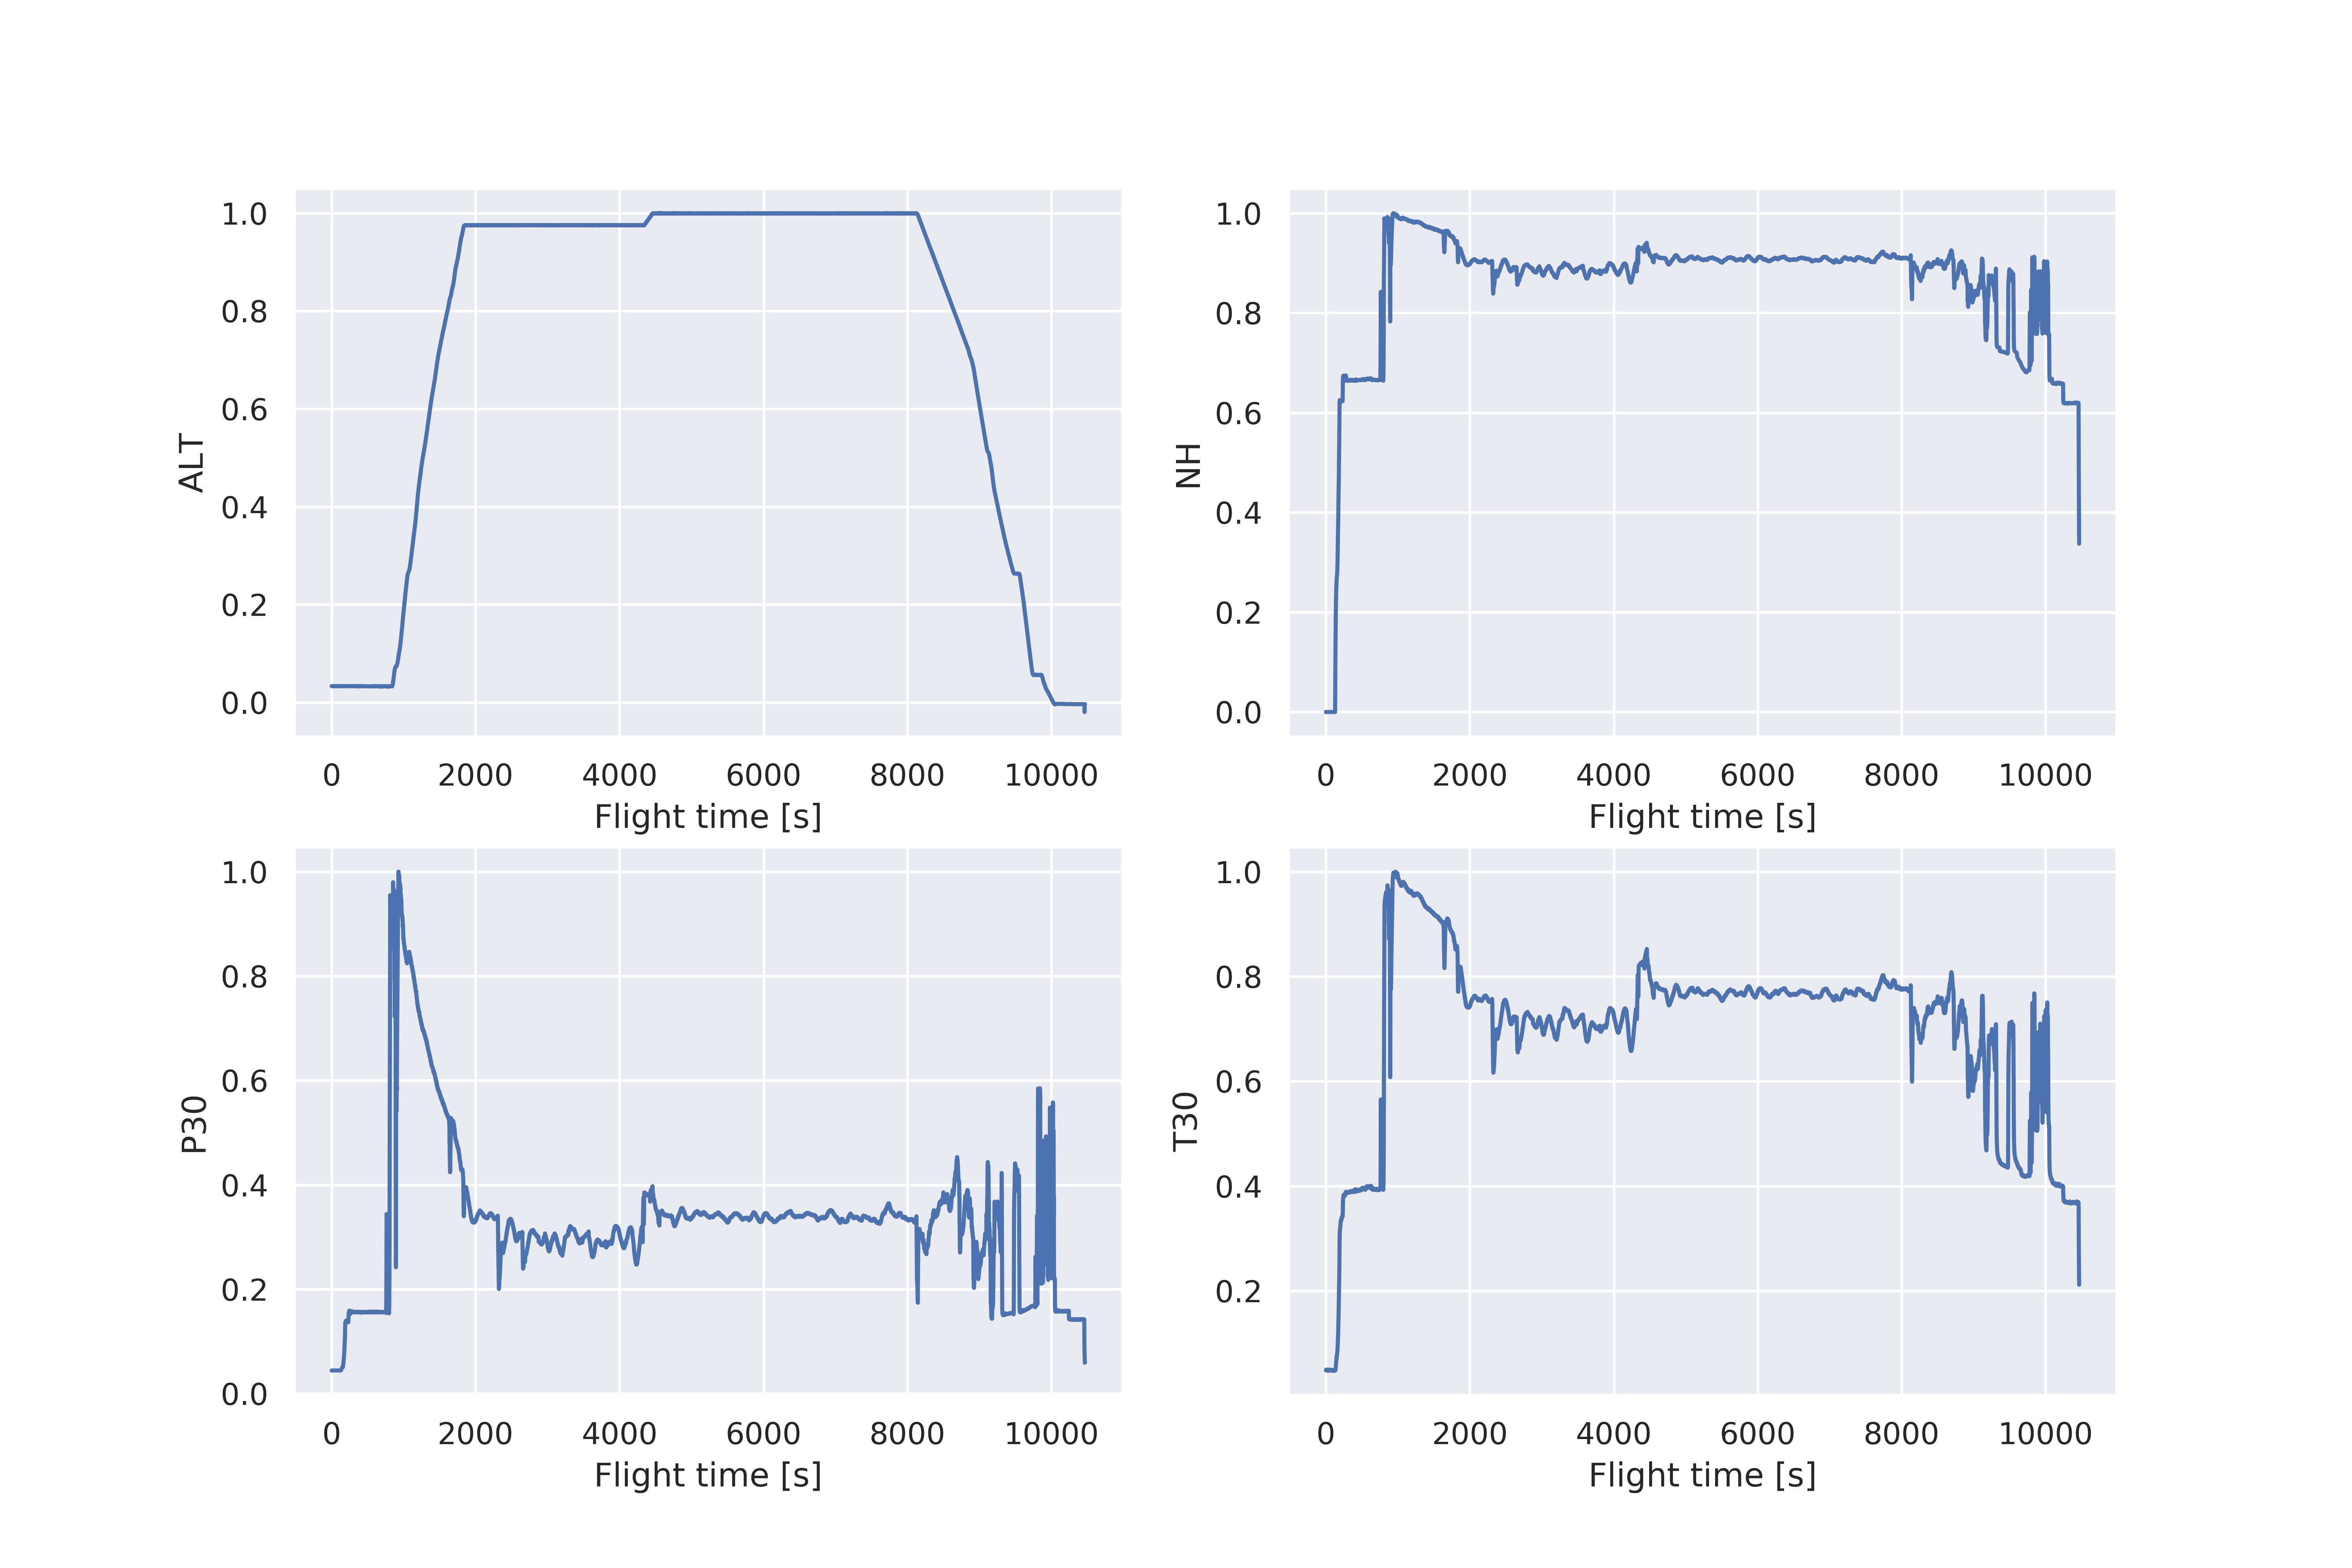
\includegraphics[width=0.95\textwidth]{6008_20150409074414}
    \caption{\label{fig:flight_example} ALT, NH, P30 and T30 of a randomly selected flight. (All parameter values normalised.)}
\end{figure}

The four flight parameters extracted from these \ac{csv} files were altitude (ALT), rotational speed of the high-pressure shaft (NH), and pressure and temperature of air exiting the compressor (P30 and T30, respectively). These values are shown (normalised) for one randomly selected flight in Figure \ref{fig:flight_example}.

NH is measured in rotations per minute, and recorded as a percentage of the maximum rotational speed defined for the engine. It therefore takes any value between 0 and 100. ALT is measured in feet; the maximum altitude across all flights was 51\,148 feet, or 15\,590 metres. P30 is measured in TODO, and ranges between 5.3 and 385.8 across all flights. The units of T30 are degrees Celsius and the values range from -12.0\textdegree{C} to 590.5\textdegree{C}.

% The majority of flights (56.6\%) reached a maximum altitude of 40\,000 feet (approximately 12\,200 metres) or higher.

\subsection{Flight Phases} \label{sec:phases}
A flight can be split into several phases: preflight, taxi out, take-off, climb, cruise, descent, reverse thrust and taxi in. These phases were extracted using internal Rolls-Royce software \cite[]{konig_br725stats_2018} that combined the flight mode parameter from \ac{ehm} data \cite[]{reischl_br700-725a1-12_2014} and custom conditions for optimisation. The conditions are summarised in table \ref{tab:flight_phases}.

The \ac{fm} often makes use of the parameter \ac{wow}, a boolean parameter with a value of 1 if the aircraft's weight is supported by its wheels, otherwise 0. Other parameters used for determining \ac{fm} include ground speed, intertial vertical speed, wing flap angle and \ac{tra}.

\begin{table}
    \begin{center}
        \caption{\label{tab:flight_phases} Summary of flight phases and conditions at which they begin \cite[]{konig_br725stats_2018}. \ac{fm} conditions in accordance with \citet{reischl_br700-725a1-12_2014}.}
        \begin{tabular}{ l l }
            Phase description & Conditions \\
            \midrule
            Preflight & \ac{fm} \(= 2\) \\
            Taxi out & left or right engine is switched on \\
            Take-off & \ac{fm} \(= 4\) \\
            % & \ac{wow} \(= 1\) \\
            % & \ac{tra} \(> 20^{\circ}\) for both engines \\
            % & ground speed \(> 28\) knots \\
            Climb & \ac{wow} \(= 0\) \\
            & intertial vertical speed \(> 500\) \(\text{ft} / \text{min}\) \\
            & altitude at least \(1500 \) m greater than at take-off \\
            Cruise & \ac{fm} \(= 6\) \\
            & altitude greater than 85\% of maximum altitude \\
            Descent & \ac{fm} \(= 7\) or \ac{fm} \(= 8\) \\
            & \ac{tra} \(< 20^{\circ} \) for both engines \\
            & Time to destination \(< 45\) \(\text{min}\) \\
            Reverse thrust & \ac{fm} \(= 9\) \\
            Taxi in & reverse thrust phase ended
        \end{tabular}
    \end{center}
\end{table}

\begin{figure}
    \centering
    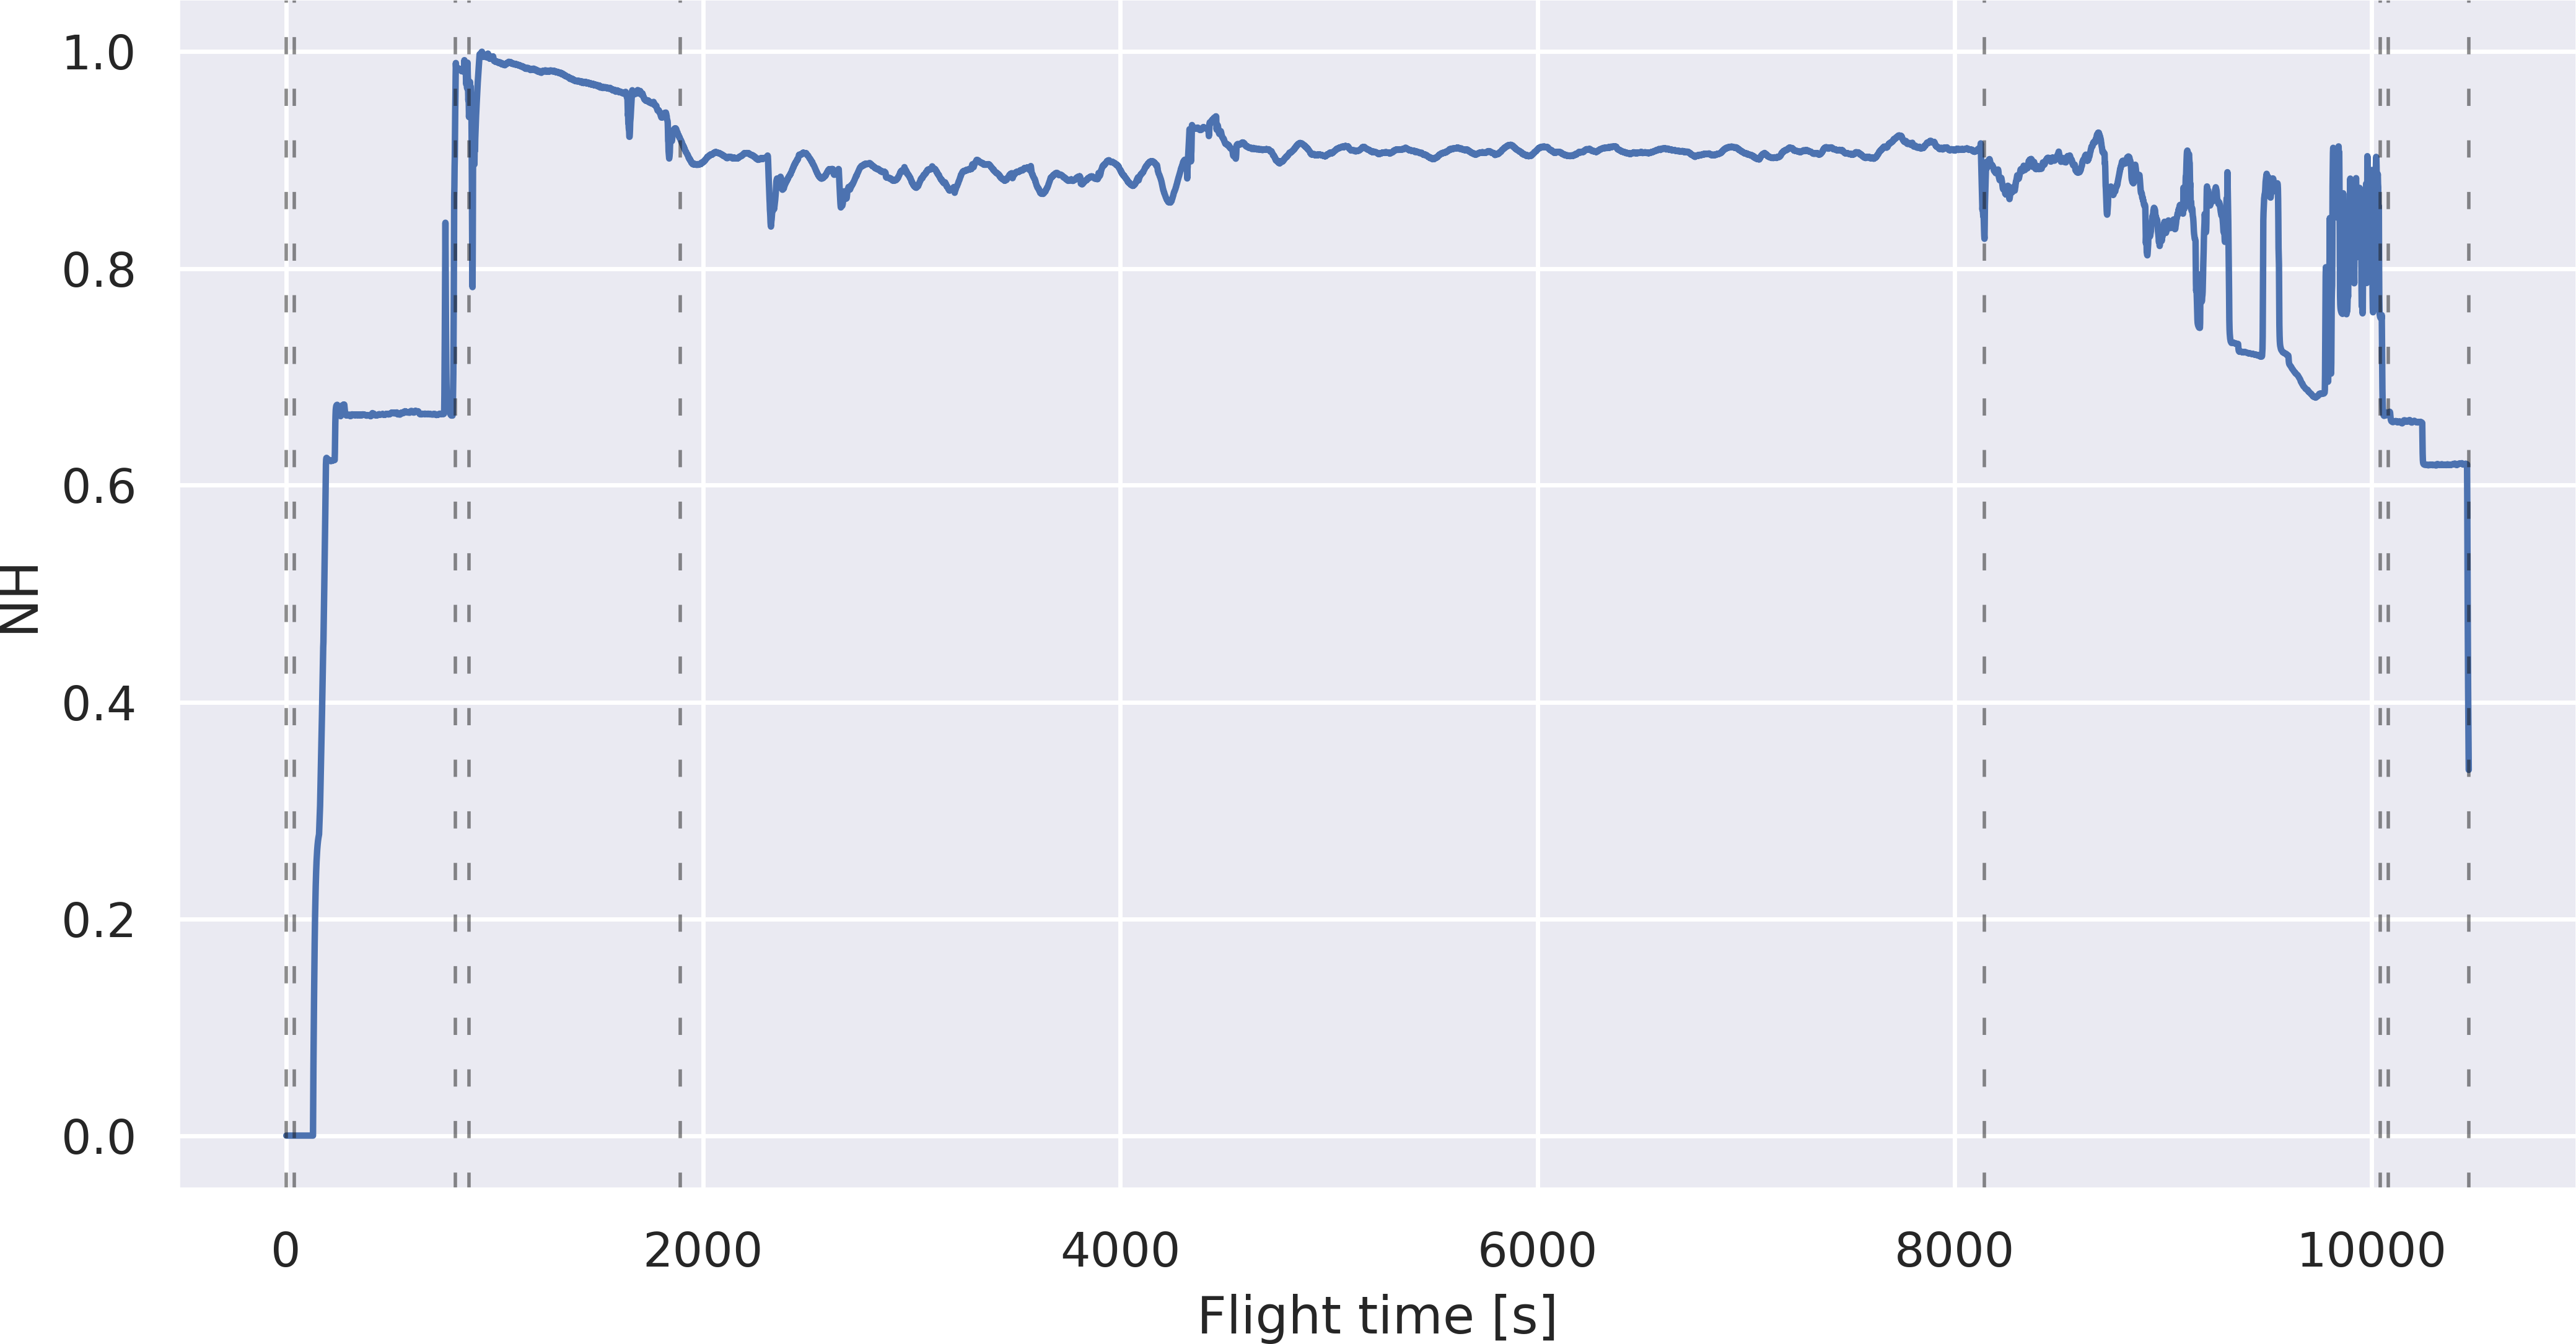
\includegraphics[width=0.95\textwidth]{6008_20150409074414_NH_phases}
    \caption{\label{fig:phases_example} Phase boundaries of NH indicated on the same flight from Figure \ref{fig:flight_example}}
\end{figure}

Figure \ref{fig:phases_example} shows the NH plot from the same flight as in Figure \ref{fig:flight_example}; dashed vertical lines represent phase boundaries.

\subsection{Features} \label{sec:features}
Seven features of the \ac{hpt} disc were selected as points of interest for the research. The features were selected based on TODO.

- 7 features selected based on

- Plot of HPT cross-section and feature locations

- 1/2 NH-driven, 4/5 P30, 6/7 T30 + plots

\begin{figure}
    \centering
    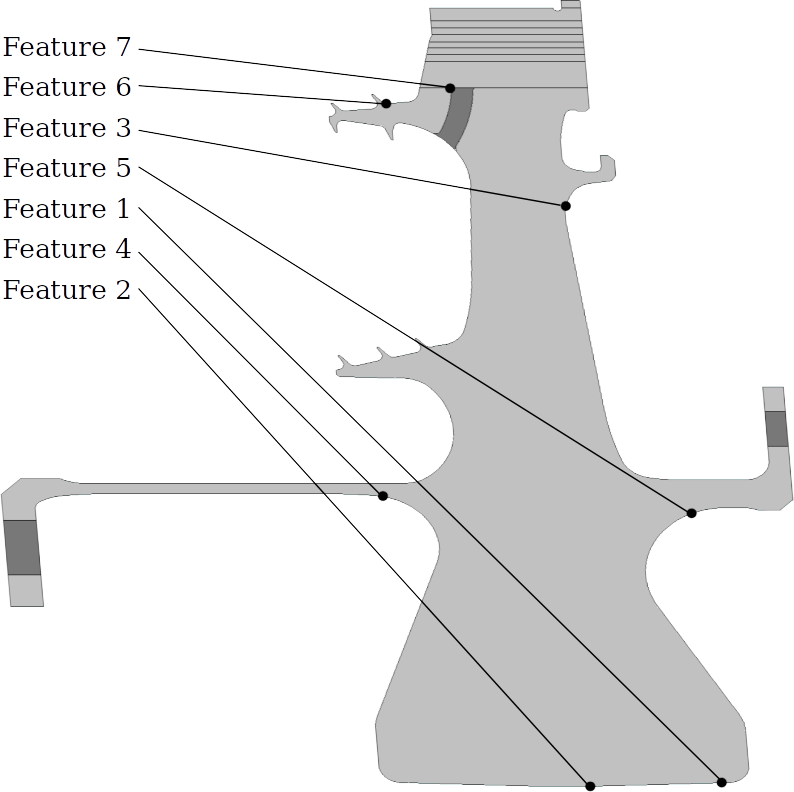
\includegraphics[width=0.6\textwidth]{hpt1_draw}
    \caption{\label{fig:hpt1} Location of features 1 to 7 on the \ac{hpt} disk. (The disk was scaled and sheared to protect intellectual property.)}
\end{figure}

\subsection{Cycle Counter} \label{sec:cyclecounter}
The \ac{ehm} data was processed using the company's internal Cycle Counter software to determine the number of cycles consumed by each feature during each flight. Figures \ref{fig:dmg_dist_low} and \ref{fig:dmg_dist_high} show the distribution of damage data (98\,315 values across 7 features from 14\,045 flights) computed by the Cycle Counter. For clarity in illustration and comparison, the distributions were split at 2 cycles: Figure \ref{fig:dmg_dist_low} contains all damage values between 0 and 2 cycles, with the overwhelming majority of the values (97\,868, 99.5\%) falling within this range; Figure \ref{fig:dmg_dist_high} contains all values above 2 cycles (with a maximum damage of 14.1 cycles), containing only 447 data points, or 0.05\%, of the total.

It should be noted that, in Figure \ref{fig:dmg_dist_low}, there are clear pairwise similarities in the distributions of the pairs mentioned in Section \ref{sec:features}. This is of no surprise, but could be highly valuable if a supervised machine learning model can be trained to use this (and other) information to extrapolate to further features.

\begin{figure}
    \centering
    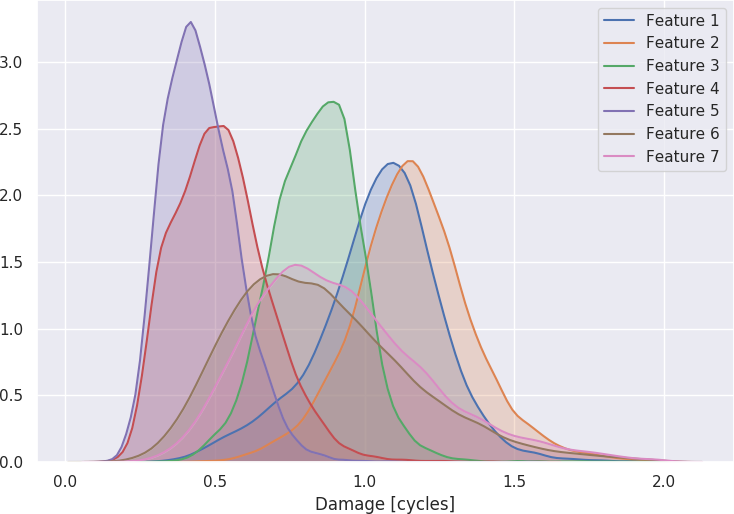
\includegraphics[width=0.95\textwidth]{distribution_low_2}
    \caption{\label{fig:dmg_dist_low} \ac{kde} plot displaying the distribution of damage cycles consumed by the seven features over 99.5\% of all 14\,045 flights (with damage of up to two cycles)}
\end{figure}

\begin{figure}
    \centering
    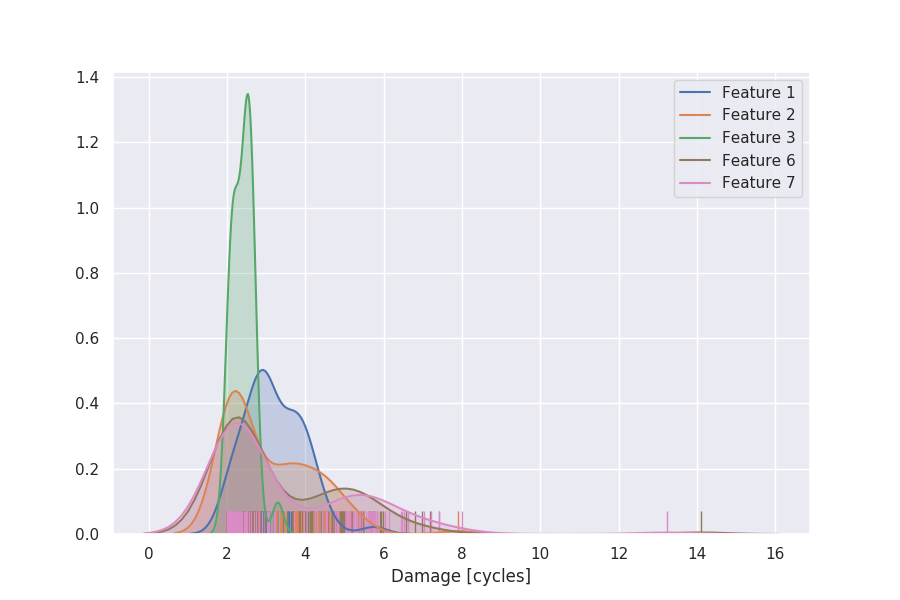
\includegraphics[width=0.95\textwidth]{distribution_high_2}
    \caption{\label{fig:dmg_dist_high} \ac{kde} plot displaying the distribution of damage cycles consumed by the seven features over 0.5\% of all 14\,045 flights (with damage of two cycles and above). The short vertical lines at the base represent individual data points. No flight caused damage of more than 2 cycles in features 4 and 5.}
\end{figure}

- Non-negligible amount of effort required to obtain this data for supervised learning. Big question: Can model scale to smaller data sets?

\subsection{Downsampling}
- Required for input layer to MLP

- Also better for scalability of models

\subsubsection{(A)PLA}

\subsubsection{APCA}

\subsubsection{Data Loss}
- Average percentage loss caused by downsampling.

- Will it affect model accuracy?

\subsection{Dataset Reduction} \label{sec:data_sizes}
The full dataset consists of \ac{ehm} data for 14\,045 flights, as well as seven Cycle Counter output values for each flight. Since scalability is an important factor in the research, the dataset was separated into two further datasets of 4\,213 and 1\,211 flights. (These three datasets will be referred to as `complete', `reduced' and `greatly reduced' datasets, respectively, in the following.)

These datasets were further split into training and validation subsets at a ratio of 3:1. The complete dataset therefore consisted of 10534 training and 3511 validation flights, the reduced dataset 3160 and 1053, and the greatly reduced dataset 909 and 302. The flights numbers in each set and subset were kept constant throughout all models to avoid skewing the data.

% \subsection{Optional: Case Studies}

% \subsubsection{6014: Stress Ranges}

% \subsubsection{6079: Long Taxi}